\title{Initial Management Report}
\author{Nicholas Grasevski \and Daniel Morton \and George El-Boustani \and Christopher Tin-Loi}
\date{\today}

\documentclass{article}
\usepackage{pdfpages}

\begin{document}
\maketitle


\section{Overview}


\section{Use Cases}
% Develop your initial use cases based on the requirements given (1
% or 2 is enough). Ask the LIC/mentor for clarifications or
% additional information.


\section{Design}
\subsection{Architecture Diagram}
% Develop an initial architecture diagram, showing the essential
% components of your system

\subsection{Interaction and Sequence Diagrams}
% Show interaction or sequence diagrams for each use case defined

\subsection{Implementation Language and Environment}
% Present and justify implementation language and environment that
% will be used


\section{Project Plan}
% Provide a project plan showing team member responsibilities, work
% arrangements and any information team members will be using to
% coordinate their activities. You should also mention any software
% tools used by the team to assist project management.

Our team is composed of four members. These are our main responsibilities throughout the project:
\begin{description}
  \item[George El Boustani] Tester
  \item[Nicholas Grasevski] Project Manager
  \item[Daniel Morton] Programmer
  \item[Christopher Tin-Loi] Programmer
\end{description}

We will be following an agile development process, with four 2-week sprints:
\begin{description}
  \item[Week 6: a working structure] By this stage, we expect to have the most simple bare bones implementation of the core system working. This excludes gui and whatnot. Currently we have coded a basic skeleton of our system, and our goal now is to fill in the stubs with the simplest working solutions. I.e. our strategy will be random, our engine will only output trades already in the file, and so on.
  \item[Week 8: a simple strategy] Once our structure is in place and working, we hope to iteratively enhance each respective component which requires improvement. This will include improving upon our basic strategy by writing other more sophisticated strategies. Other components of our Algorithmic Trading System will be addressed too. We plan to improve the trading engine incrementally to handle orders in a more realistic manner, and we also plan to improve the strategy evaluator by expanding on the generated evaluation report.
  \item[Week 10: public demo] By this stage we should have our graphical user interface, and it should be streamlined and intuitive for the user.
  \item[Week 12: final demo] By this stage we should have polished all components to an acceptable level.
\end{description}

The project schedule can be found in the appendix. We are currently at the beginning of the first sprint.

We are using various software tools to coordinate our work and to aid in project management:
\begin{description}
  \item[Communication] Currently we communicate primarily through email. Communicating through email gives us a historical record of our interactions and decisions. We also have weekly face to face meetings, phone and sms communication and internet relay chat communications.
  \item[Version Control] We are using the git VCS to keep track of changes to our code. It allows us to collaborate on our source code tree and record each version. However we havent limited this to source code and are in fact recording all work including documentation and reports in git, so that we have a record of every change.
  \item[Build System] We also have a build script which compiles all of our source code and documentation and runs all of our tests. We have added this as a pre-commit hook, so that every time somebody commits, all of the documentation is regenerated and all of the tests are run. If any of these steps fail, the commit is rejected. This acts as a sanity check that mitigates the risk of somebody pushing buggy code to the repository. It also ensures that our documentation is kept up to date.
  \item[Source Code Hosting] We have set up a repository on github to enable easier collaboration between our own respective local repositories. We have gone with a centralized model because we are a small team and want to keep things simple. Ideally each of us will regularly pull each others changes from this repository and push our own changes.
  \item[Issue Tracker] In addition to git hosting, github also provides some basic project management tools. One of these is the issue tracker, which allows one to track feature requests, bugs, milestones and so on. We are currently using this in conjunction with the Gantt chart to track our progress in each sprint, and perhaps in the later stages of development to alert team members of bugs and new requirements. The issue tracker also provides a place to document each task and the ability to comment on an issue provides a record of design decisions made, as well as a concrete interpretation of the requirement.
  \item[Wiki] Github also provides wiki hosting for each project, so we may use this if we find a use for it.
  \item[Code Review] Github enables team members to comment on commits and on tasks, so if a team member finds some dodgy source code, they can either comment on the commit where that dodgy code was introduced or they can comment on the corresponding task in the issue tracker. The culprit is then automatically notified, and they can also respond with a justification for why the code is that way if appropriate.
\end{description}


\section{Summary}


\appendix
\section{Project Schedule}
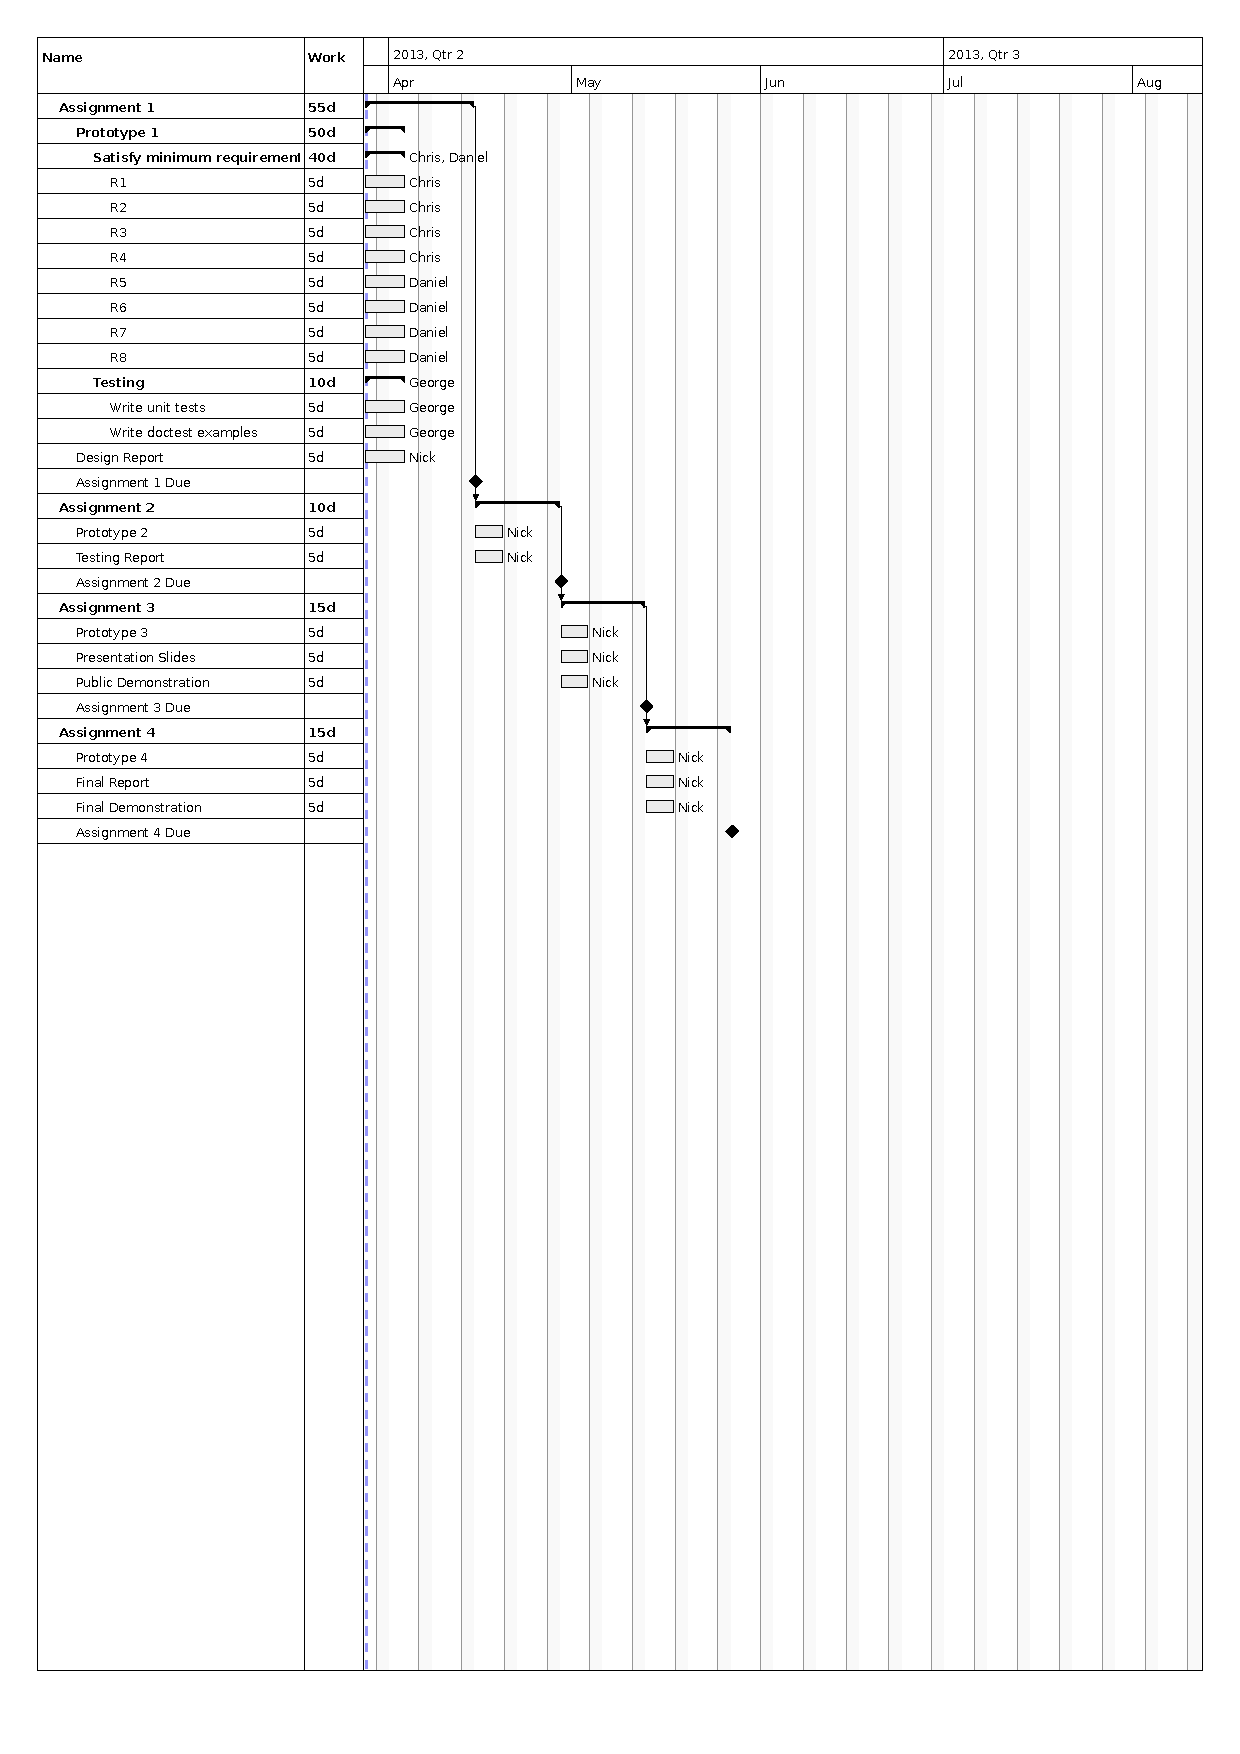
\includepdf[pages={-}]{schedule}

\end{document}
